% ============================================================================
% Ouroboros IDS — Documentación del Proyecto Final
% Universidad Autónoma de Aguascalientes
% Seguridad en Sistemas — 8°B
%
% Formato: estilo IEEE (tipografía Times, figuras "Fig. N", encabezados
% jerárquicos numerados). Bibliografía en formato APA conforme a la rúbrica.
%
% Compilar con: pdflatex (2 pasadas para índices) o en Overleaf.
% Colocar el logotipo institucional como docs/logo_uaa.png
% ============================================================================
\documentclass[12pt,letterpaper]{report}

\usepackage[utf8]{inputenc}
\usepackage[T1]{fontenc}
% Babel español si está disponible (Overleaf / TeX Live completo);
% si no, nombres en español definidos manualmente.
\IfFileExists{spanish.ldf}
  {\usepackage[spanish,es-tabla]{babel}}
  {\AtBeginDocument{%
     \renewcommand{\contentsname}{Índice general}%
     \renewcommand{\listfigurename}{Índice de figuras}%
     \renewcommand{\listtablename}{Índice de tablas}%
     \renewcommand{\chaptername}{Capítulo}%
     \renewcommand{\abstractname}{Resumen}%
     \renewcommand{\figurename}{Fig.}%
     \renewcommand{\tablename}{Tabla}%
   }}
\usepackage{mathptmx}                 % Tipografía Times (estilo IEEE)
\usepackage[margin=2.5cm]{geometry}
\usepackage{graphicx}
\usepackage{float}
\usepackage{booktabs}
\usepackage{array}
\usepackage{longtable}
\usepackage{enumitem}
\usepackage{tikz}
\usetikzlibrary{shapes.geometric, arrows.meta, positioning}
\usepackage{caption}
\captionsetup[figure]{name=Fig.,labelsep=period,font=small}
\captionsetup[table]{name=Tabla,labelsep=period,font=small}
\usepackage{listings}
\usepackage{xcolor}
\usepackage[hidelinks]{hyperref}
\usepackage{setspace}

% ── Estilo de código ─────────────────────────────────────────────────────────
\definecolor{fondocodigo}{RGB}{245,245,245}
\lstset{
  basicstyle=\ttfamily\small,
  backgroundcolor=\color{fondocodigo},
  frame=single, framerule=0.3pt,
  breaklines=true,
  showstringspaces=false,
  literate={á}{{\'a}}1 {é}{{\'e}}1 {í}{{\'i}}1 {ó}{{\'o}}1 {ú}{{\'u}}1
           {ñ}{{\~n}}1 {Á}{{\'A}}1 {É}{{\'E}}1 {Í}{{\'I}}1 {Ó}{{\'O}}1
           {Ú}{{\'U}}1 {Ñ}{{\~N}}1
}

% ── Estilos TikZ para el diagrama de flujo ───────────────────────────────────
\tikzset{
  proceso/.style={rectangle, rounded corners=2pt, draw=black, fill=gray!10,
                  text width=4.2cm, minimum height=0.9cm, align=center,
                  font=\small},
  decision/.style={diamond, aspect=2.2, draw=black, fill=gray!20,
                   text width=3.2cm, align=center, font=\small, inner sep=1pt},
  almacen/.style={rectangle, draw=black, fill=blue!8, text width=4.2cm,
                  minimum height=0.9cm, align=center, font=\small},
  alerta/.style={rectangle, rounded corners=2pt, draw=red!60!black,
                 fill=red!10, text width=4.2cm, minimum height=0.9cm,
                 align=center, font=\small},
  flecha/.style={-{Stealth[length=2.5mm]}, thick}
}

\begin{document}

% ============================================================================
% PORTADA
% ============================================================================
\begin{titlepage}
  \centering
  % Logotipo institucional — colocar el archivo logo_uaa.png junto al .tex
  \IfFileExists{logo_uaa.png}
    {\includegraphics[width=4.5cm]{logo_uaa.png}}
    {\fbox{\parbox[c][3.5cm][c]{4.5cm}{\centering Logotipo\\UAA}}}

  \vspace{0.8cm}
  {\Large \textbf{Universidad Autónoma de Aguascalientes}}\\[0.25cm]
  {\large Centro de Ciencias Básicas}\\[0.15cm]
  {\large Ingeniería en Sistemas Computacionales}\\[0.15cm]
  {\large Seguridad en Sistemas --- 8\textsuperscript{o}~B}

  \vspace{1.6cm}
  \rule{\textwidth}{0.6pt}\\[0.55cm]
  {\LARGE \textbf{Ouroboros IDS}}\\[0.35cm]
  {\Large Sistema de Detección de Intrusos para Redes\\Institucionales con
   Análisis Forense Automatizado}\\[0.45cm]
  {\large \textit{Proyecto Final}}\\[0.4cm]
  \rule{\textwidth}{0.6pt}

  \vspace{1.6cm}
  {\large \textbf{Integrantes}}\\[0.3cm]
  {\large Daan Jostin Carabez García}\\[0.15cm]
  {\large Diego Iván Salas Pedroza}\\[0.15cm]
  {\large Jaime Iván López Gutiérrez}

  \vspace{1.4cm}
  {\large \textbf{Profesor:} Arturo Ocampo Silva}

  \vfill
  {\large Aguascalientes, Ags. --- Junio de 2026}
\end{titlepage}

% ============================================================================
% ÍNDICES (automatizados)
% ============================================================================
\tableofcontents
\listoffigures
\listoftables
\newpage

% ============================================================================
% RESUMEN
% ============================================================================
\begin{abstract}
\noindent
Ouroboros es un Sistema de Detección de Intrusos (IDS) de red desarrollado en
Python para redes locales institucionales sobre GNU/Linux. Captura tráfico en
tiempo real mediante Scapy, mantiene una lista blanca dinámica de dispositivos
por dirección MAC (Capa 2) e IP (Capa 3), registra las consultas DNS de los
usuarios, detecta conexiones hacia IPs asociadas a malware mediante una lista
negra alimentada por \textit{feeds} de \textit{Threat Intelligence}, y ante
cada incidente notifica al administrador por correo electrónico con un
reporte forense automatizado que incluye resolución DNS inversa (rDNS),
categorías de ataque decodificadas (taxonomía de 23 categorías de AbuseIPDB),
score de abuso, historial de reportes, geolocalización y WHOIS. El sistema
se administra mediante un \textit{dashboard} web con autenticación JWT,
control de acceso por roles y una CLI. Este documento integra el manual de
usuario, la documentación de arquitectura, las medidas de protección de
credenciales y el análisis jurídico del monitoreo conforme a la legislación
mexicana vigente.\\[0.3cm]
\textbf{Palabras clave:} IDS, Scapy, lista blanca, \textit{threat
intelligence}, análisis forense, JWT, LFPDPPP.
\end{abstract}

% ============================================================================
\chapter{Introducción}
% ============================================================================

Toda organización necesita controlar la información que fluye por su
infraestructura de manera ágil, detectando comportamientos anómalos antes de
que se conviertan en incidentes de difícil contención. Ouroboros IDS responde
a esa necesidad: es un sistema de detección de intrusos pasivo que vigila la
red local, identifica dispositivos no autorizados, registra los sitios que
visitan los usuarios y reacciona ante conexiones hacia infraestructura
maliciosa conocida, automatizando tanto la notificación como la recolección
de evidencia forense.

\section{Objetivo general}
Desarrollar un IDS funcional para redes locales que valide dispositivos
contra una lista blanca (Capas 2 y 3 del modelo OSI), genere una bitácora de
sitios visitados, detecte conexiones a IPs peligrosas mediante listas negras
con \textit{feeds} de \textit{Threat Intelligence}, y automatice el análisis
forense y la notificación al administrador por correo electrónico.

\section{Alcance y sistema operativo objetivo}
El sistema está diseñado para implementarse en \textbf{GNU/Linux} (probado en
distribuciones basadas en Debian/Ubuntu). La captura de paquetes requiere
\texttt{libpcap} y privilegios de superusuario. El \textit{dashboard} web y
la CLI de consulta funcionan sin privilegios elevados y pueden accederse
desde cualquier dispositivo de la red local.

\section{Licenciamiento}
En congruencia con la filosofía del software libre promovida por Richard
Stallman y Linus Torvalds, el proyecto se desarrolló con la intención de
distribuirse bajo licencia GNU/GPL: el código se comparte, se documenta y
puede ser auditado por terceros, sin que ello comprometa las credenciales ni
los datos operativos del sistema (véase el Capítulo~\ref{cap:seguridad}).

% ============================================================================
\chapter{Arquitectura del sistema y Modelo OSI}
% ============================================================================

\section{Stack tecnológico}

\begin{table}[H]
\centering
\caption{Stack tecnológico de Ouroboros IDS.}
\label{tab:stack}
\begin{tabular}{ll}
\toprule
\textbf{Componente} & \textbf{Tecnología} \\
\midrule
Captura de paquetes        & Scapy \\
Base de datos              & SQLite (modo WAL) \\
\textit{Dashboard} web     & Flask + PyJWT + Werkzeug \\
Correo                     & \texttt{smtplib} (SMTP/TLS) \\
\textit{Threat Intelligence} & AbuseIPDB API (taxonomía de 23 categorías), ip-api.com,
                               python-whois, \texttt{socket} (DNS inverso / rDNS) \\
Detección de red           & netifaces, ARP scan activo \\
Configuración              & python-dotenv (\texttt{.env}) \\
Instalación                & \texttt{pyproject.toml} (setuptools) \\
\bottomrule
\end{tabular}
\end{table}

\section{Módulos y capas del Modelo OSI}

Ouroboros opera sobre varias capas del modelo OSI de manera simultánea, como
se muestra en la Tabla~\ref{tab:osi}.

\begin{table}[H]
\centering
\caption{Correspondencia entre módulos de Ouroboros y capas del modelo OSI.}
\label{tab:osi}
\begin{tabular}{cll}
\toprule
\textbf{Capa OSI} & \textbf{Protocolo} & \textbf{Función en Ouroboros} \\
\midrule
2 (Enlace)     & ARP  & Lista blanca por dirección MAC; ARP scan activo \\
3 (Red)        & IP   & Validación de origen autorizado y destino peligroso \\
4 (Transporte) & TCP/UDP & Extracción de puerto de destino y protocolo de cada
                            paquete que genera una alerta de lista negra \\
7 (Aplicación) & DNS  & Bitácora de dominios visitados por los usuarios \\
7 (Aplicación) & SMTP & Notificación de alertas al administrador \\
7 (Aplicación) & HTTP & \textit{Dashboard} de administración y \textit{feeds} \\
\bottomrule
\end{tabular}
\end{table}

\section{Diagrama de flujo del sistema}

La Fig.~\ref{fig:flujo} muestra el flujo de detección completo: el
\textit{sniffer} captura cada paquete y lo procesa por capas; las alertas se
persisten en SQLite y un hilo \textit{worker} independiente las procesa cada
5 segundos, enviando los correos y ejecutando el análisis forense.

\begin{figure}[H]
\centering
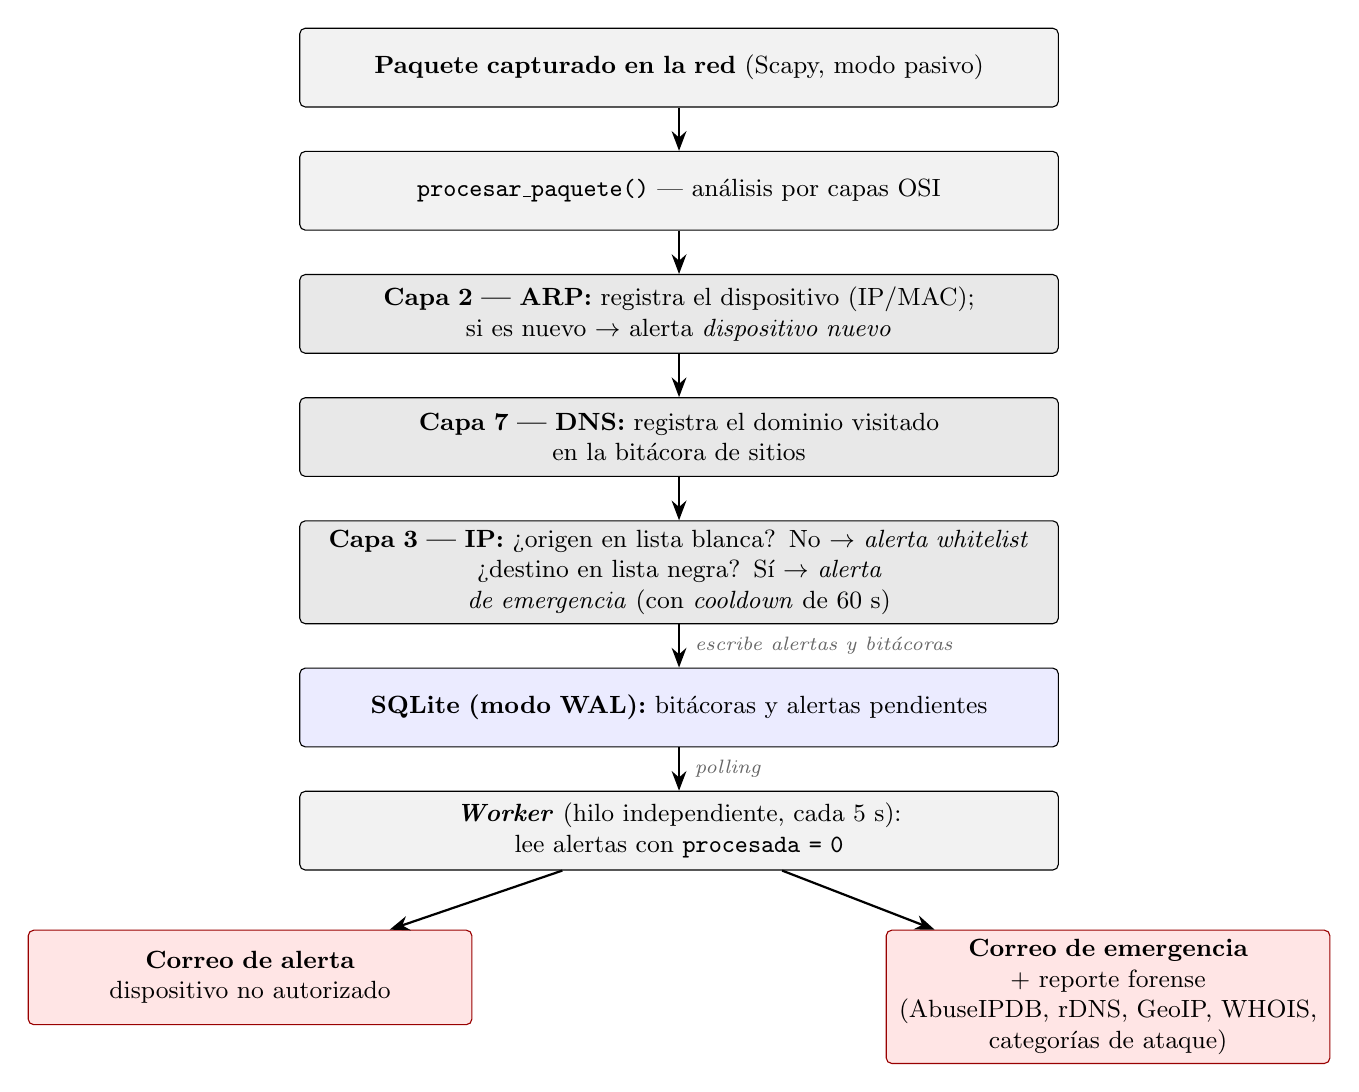
\begin{tikzpicture}[
  caja/.style={rectangle, rounded corners=2pt, draw=black, fill=gray!10,
               text width=9.4cm, minimum height=1.0cm, align=center,
               font=\small},
  capa/.style={caja, fill=gray!18},
  datos/.style={caja, fill=blue!8},
  correo/.style={rectangle, rounded corners=2pt, draw=red!60!black,
                 fill=red!10, text width=5.4cm, minimum height=1.2cm,
                 align=center, font=\small},
  etiqueta/.style={font=\scriptsize\itshape, text=black!60},
  flecha/.style={-{Stealth[length=2.5mm]}, thick}
]
  % ── Pipeline vertical (sin cruces) ──
  \node[caja]                       (paq)    at (0,0)
        {\textbf{Paquete capturado en la red} (Scapy, modo pasivo)};
  \node[caja, below=0.55cm of paq]  (proc)
        {\texttt{procesar\_paquete()} --- análisis por capas OSI};
  \node[capa, below=0.55cm of proc] (arp)
        {\textbf{Capa 2 --- ARP:} registra el dispositivo (IP/MAC);\\
         si es nuevo $\rightarrow$ alerta \textit{dispositivo nuevo}};
  \node[capa, below=0.55cm of arp]  (dns)
        {\textbf{Capa 7 --- DNS:} registra el dominio visitado\\
         en la bitácora de sitios};
  \node[capa, below=0.55cm of dns]  (ip)
        {\textbf{Capa 3 --- IP:} ¿origen en lista blanca?
         No $\rightarrow$ \textit{alerta whitelist}\\
         ¿destino en lista negra? Sí $\rightarrow$ \textit{alerta de
         emergencia} (con \textit{cooldown} de 60 s)};
  \node[datos, below=0.55cm of ip]  (bd)
        {\textbf{SQLite (modo WAL):} bitácoras y alertas pendientes};
  \node[caja, below=0.55cm of bd]   (worker)
        {\textbf{\textit{Worker}} (hilo independiente, cada 5 s):\\
         lee alertas con \texttt{procesada = 0}};
  \node[correo, below left=0.75cm and -2.2cm of worker]  (correo1)
        {\textbf{Correo de alerta}\\dispositivo no autorizado};
  \node[correo, below right=0.75cm and -2.2cm of worker] (correo2)
        {\textbf{Correo de emergencia}\\+ reporte forense\\
         (AbuseIPDB, rDNS, GeoIP, WHOIS,\\categorías de ataque)};

  % ── Flechas del pipeline ──
  \draw[flecha] (paq)    -- (proc);
  \draw[flecha] (proc)   -- (arp);
  \draw[flecha] (arp)    -- (dns);
  \draw[flecha] (dns)    -- (ip);
  \draw[flecha] (ip)     -- node[etiqueta, right=2pt] {escribe alertas y bitácoras} (bd);
  \draw[flecha] (bd)     -- node[etiqueta, right=2pt] {\textit{polling}} (worker);
  \draw[flecha] (worker) -- (correo1);
  \draw[flecha] (worker) -- (correo2);
\end{tikzpicture}
\caption{Diagrama de flujo de detección y notificación de Ouroboros IDS.}
\label{fig:flujo}
\end{figure}

\section{Estructura de archivos}

\begin{lstlisting}
ouroboros-ids/
|- ouroboros.py          # Punto de entrada principal (sudo)
|- cli.py                # CLI de administracion (sin sudo)
|- seed_demo.py          # Generador de datos de prueba
|- pyproject.toml        # Configuracion del paquete
|- .env                  # Credenciales (NO versionado)
|- config/settings.py    # Configuracion central
|- core/
|  |- sniffer.py         # Motor de captura (Scapy)
|  |- blacklist.py       # Gestion de lista negra
|  |- db_writer.py       # Capa de acceso a SQLite
|  |- feed_updater.py    # Descarga de feeds remotos
|- services/
|  |- worker.py          # Procesamiento de alertas (hilo)
|  |- mailer.py          # Correos HTML
|  |- abuse_api.py       # AbuseIPDB / GeoIP / WHOIS
|  |- logger.py          # Bitacora en archivo
|- dashboard/dashboard.py # Dashboard web (Flask + JWT)
|- data/
   |- ouroboros.db       # Base de datos SQLite
   |- blacklist.txt      # Lista negra local
\end{lstlisting}

\section{Base de datos}

\begin{table}[H]
\centering
\caption{Tablas de la base de datos SQLite.}
\label{tab:tablas}
\begin{tabular}{lp{8.6cm}}
\toprule
\textbf{Tabla} & \textbf{Descripción} \\
\midrule
\texttt{dispositivos\_conocidos} & Cada MAC vista en la red, con IP,
  marcas de tiempo y bandera de autorización (lista blanca dinámica). \\
\texttt{alertas\_whitelist} & Alertas por dispositivos no autorizados. \\
\texttt{bitacora\_dns} & Dominios consultados por cada IP de la red. \\
\texttt{alertas\_blacklist} & Conexiones detectadas hacia IPs peligrosas, con
  IP/MAC de origen, IP peligrosa, \textbf{puerto de destino y protocolo}
  (TCP/UDP/otro) extraídos del paquete que generó la alerta. \\
\texttt{feed\_sources} & Fuentes remotas de \textit{Threat Intelligence}. \\
\texttt{analisis\_forense} & Inteligencia por IP peligrosa: score de abuso
  (0--100), tipo de riesgo, \textbf{hostname por DNS inverso} (rDNS),
  \textbf{total de reportes} en AbuseIPDB y fecha del último, \textbf{categorías
  de ataque} decodificadas (taxonomía de 23 categorías de AbuseIPDB), país,
  ISP y correo de abuso del proveedor. \\
\texttt{usuarios} & Cuentas del \textit{dashboard} (hash PBKDF2, rol,
  bandera de contraseña temporal). \\
\bottomrule
\end{tabular}
\end{table}

% ============================================================================
\chapter{Manual de usuario}
% ============================================================================

\textbf{Sistema operativo de implementación: GNU/Linux} (recomendado
Ubuntu/Debian). El \textit{dashboard} puede consultarse desde cualquier
dispositivo con navegador en la misma red.

\section{Guía de instalación y requisitos}

\subsection{Requisitos de hardware y software}
\begin{itemize}[nosep]
  \item Equipo con GNU/Linux conectado a la red a monitorear (idealmente por
        cable, con la interfaz en modo promiscuo).
  \item Python 3.10 o superior.
  \item \texttt{libpcap} --- biblioteca de captura de paquetes que utiliza
        Scapy en Linux (en Windows el equivalente sería Npcap; no soportado
        por el \textit{sniffer} de Ouroboros).
  \item Acceso a Internet para los \textit{feeds} de \textit{Threat
        Intelligence} y las APIs forenses.
  \item Cuenta de correo con SMTP habilitado (probado con Gmail).
  \item API key gratuita de AbuseIPDB (\url{https://www.abuseipdb.com}).
\end{itemize}

\subsection{Instalación de dependencias del sistema}
\begin{lstlisting}[language=bash]
sudo apt update
sudo apt install python3 python3-venv python3-pip libpcap0.8 git
\end{lstlisting}

\subsection{Instalación de Ouroboros}
\begin{lstlisting}[language=bash]
git clone https://github.com/<equipo>/ouroboros-ids.git
cd ouroboros-ids
python3 -m venv venv
source venv/bin/activate
pip install -e .
\end{lstlisting}

Esto instala automáticamente las dependencias declaradas en
\texttt{pyproject.toml}: Flask, PyJWT, Werkzeug, netifaces2, python-dotenv,
requests, scapy y python-whois.

\subsection{Configuración del servidor SMTP y credenciales}
\label{sec:smtp}

Copiar la plantilla y editar las variables:
\begin{lstlisting}[language=bash]
cp .env.example .env
nano .env
\end{lstlisting}

\begin{lstlisting}
SMTP_EMAIL=correo@gmail.com
SMTP_PASSWORD=contrasena_de_aplicacion
SMTP_HOST=smtp.gmail.com
SMTP_PORT=587
ADMIN_EMAIL=admin@dominio.com
ABUSEIPDB_KEY=tu_api_key
DB_PATH=data/ouroboros.db
\end{lstlisting}

\textbf{Importante (Gmail):} no se usa la contraseña normal de la cuenta.
Debe generarse una \textit{contraseña de aplicación}: activar verificación en
dos pasos en \url{https://myaccount.google.com/security} y después crear una
contraseña de aplicación en \textit{Contraseñas de aplicaciones}. Esa cadena
de 16 caracteres es la que va en \texttt{SMTP\_PASSWORD}.

\section{Instrucciones de operación}

\subsection{Arranque del sistema}
\begin{lstlisting}[language=bash]
sudo ouroboros                  # deteccion automatica de interfaz
sudo ouroboros --interface eth0 # interfaz especifica
\end{lstlisting}

Al arrancar, el sistema: valida las variables de entorno, detecta la
interfaz, inicializa la base de datos, descarga los \textit{feeds} de la
lista negra, ejecuta un ARP scan para poblar la lista de dispositivos,
levanta el \textit{worker} de alertas y el \textit{dashboard} web, y queda
capturando tráfico hasta \texttt{Ctrl+C}.

\begin{figure}[H]
\centering
\fbox{\parbox[c][5.2cm][c]{0.85\textwidth}{\centering\itshape
  [Insertar captura: terminal con el arranque de \texttt{sudo ouroboros},
  mostrando el banner, el ARP scan y los hilos iniciados]}}
\caption{Arranque del IDS en terminal.}
\label{fig:arranque}
\end{figure}

\subsection{Acceso al dashboard y primer inicio de sesión}

Desde un navegador en la misma red:
\texttt{http://<IP-del-servidor>:5000}. Iniciar sesión con el usuario
administrador inicial. \textbf{En el primer acceso el sistema obliga a
cambiar la contraseña} (mínimo 8 caracteres) antes de poder usar cualquier
vista; esto aplica también a toda cuenta nueva que cree el administrador.

\begin{figure}[H]
\centering
\fbox{\parbox[c][5.2cm][c]{0.85\textwidth}{\centering\itshape
  [Insertar captura: pantalla de login del dashboard]}}
\caption{Pantalla de inicio de sesión con autenticación JWT.}
\label{fig:login}
\end{figure}

\subsection{Alta de un dispositivo en la lista blanca (IP/MAC)}
\label{sec:altamac}

La lista blanca vive en la tabla \texttt{dispositivos\_conocidos} y se
gestiona por dirección MAC (la IP puede cambiar por DHCP; el \textit{sniffer}
la actualiza automáticamente). Hay tres formas de dar de alta un equipo:

\begin{enumerate}[nosep]
  \item \textbf{Autorizar uno detectado:} en la vista
        \textit{Dispositivos}, todo equipo visto en la red aparece como
        \textit{No autorizado}; basta pulsar el botón \textbf{Autorizar}.
  \item \textbf{Alta manual por MAC:} en la misma vista, capturar la MAC en
        el formato \texttt{AA:BB:CC:DD:EE:FF} y pulsar
        \textbf{Autorizar MAC}.
  \item \textbf{Por CLI (sin sudo):}
\begin{lstlisting}[language=bash]
ouroboros devices list
ouroboros devices authorize AA:BB:CC:DD:EE:FF
\end{lstlisting}
\end{enumerate}

\begin{figure}[H]
\centering
\fbox{\parbox[c][5.2cm][c]{0.85\textwidth}{\centering\itshape
  [Insertar captura: vista Dispositivos con el formulario de alta por MAC y
  los botones Autorizar]}}
\caption{Alta y autorización de dispositivos en la lista blanca.}
\label{fig:whitelist}
\end{figure}

\subsection{Consulta del reporte de sitios visitados}

La vista \textit{Bitácora DNS} muestra en tiempo real los dominios que
consulta cada dispositivo, con filtro por IP de origen. El resumen inicial
incluye el \textit{top} de dominios más visitados. Desde la CLI:
\texttt{ouroboros dns <ip>}.

\begin{figure}[H]
\centering
\fbox{\parbox[c][5.2cm][c]{0.85\textwidth}{\centering\itshape
  [Insertar captura: vista Bitácora DNS con dominios visitados]}}
\caption{Reporte en tiempo real de dominios visitados.}
\label{fig:dns}
\end{figure}

\subsection{Interpretación de las alertas}

\begin{table}[H]
\centering
\caption{Tipos de correo que envía Ouroboros y cómo interpretarlos.}
\label{tab:alertas}
\begin{tabular}{p{4.6cm}p{9.2cm}}
\toprule
\textbf{Asunto del correo} & \textbf{Significado y acción recomendada} \\
\midrule
\texttt{[Ouroboros] Alerta --- Dispositivo no autorizado} &
Un equipo cuya MAC no está en la lista blanca generó tráfico. Verificar
físicamente el dispositivo; si es legítimo, autorizarlo desde el
\textit{dashboard}; si no, investigar posible intrusión. \\
\midrule
\texttt{[Ouroboros] EMERGENCIA --- Conexión a IP peligrosa} &
Un dispositivo interno se comunicó con una IP de la lista negra. El correo
especifica el tipo de riesgo (ej. \textit{Botnet/C2, Malware}). Aislar el
equipo de la red y analizarlo con antivirus. \\
\midrule
\texttt{[Ouroboros] Reporte Forense --- <ip>} &
Resultado del análisis automatizado: \textbf{hostname por DNS inverso} (rDNS),
score de abuso (0--100), total de reportes previos en AbuseIPDB y fecha del
último, \textbf{categorías de ataque} (ej.\ \textit{Brute-Force, Port Scan,
SSH}), país, ISP y \textbf{correo de abuso del proveedor}, listo para
reenviar la denuncia al proveedor del host malicioso. \\
\bottomrule
\end{tabular}
\end{table}

En el \textit{dashboard}, la tarjeta \textit{Alertas IP peligrosa} del
resumen se enciende en rojo pulsante cuando existen detecciones, y cada
tarjeta funciona como atajo a su vista correspondiente.

\begin{figure}[H]
\centering
\fbox{\parbox[c][5.2cm][c]{0.85\textwidth}{\centering\itshape
  [Insertar captura: correo de emergencia recibido + reporte forense]}}
\caption{Correo de alerta de emergencia con análisis forense.}
\label{fig:correo}
\end{figure}

\subsection{Gestión de la lista negra y los feeds}

En la vista \textit{IPs Peligrosas}, la pestaña \textit{Lista local} permite
agregar/quitar IPs de \texttt{blacklist.txt}, y la pestaña \textit{Feeds
remotos} administra las fuentes de \textit{Threat Intelligence} (Feodo
Tracker, Emerging Threats, Tor Exit Nodes, CINS). Todo cambio se aplica
\textbf{en caliente}: el \textit{sniffer} recarga la lista en
$\sim$5 segundos sin reiniciar, mediante un archivo-señal.

\subsection{Gestión de cuentas}

La vista \textit{Usuarios} (solo rol \texttt{admin}) permite crear cuentas
con contraseña temporal y rol \texttt{operador} o \texttt{admin}. El correo
del administrador que recibe las alertas se cambia en
\textit{Configuración}, protegido por el esquema de identificación
(usuario), autenticación (JWT firmado) y autorización (rol \texttt{admin}).

\section{Troubleshooting básico}

\begin{table}[H]
\centering
\caption{Errores comunes y soluciones.}
\label{tab:trouble}
\begin{tabular}{p{4.8cm}p{9.0cm}}
\toprule
\textbf{Problema} & \textbf{Causa y solución} \\
\midrule
\textbf{El correo de alerta llega a spam} &
Los filtros penalizan correos automatizados con asuntos de urgencia. (1)
Marcar el primer correo como \textit{No es spam}; (2) agregar
\texttt{SMTP\_EMAIL} a los contactos del administrador; (3) crear un filtro
en Gmail: \textit{De: <correo del sistema>} $\rightarrow$ \textit{Nunca
enviar a spam}; (4) en dominios propios, configurar registros SPF/DKIM del
remitente. \\
\midrule
\texttt{PermissionError} o \texttt{Operation not permitted} al arrancar &
La captura de paquetes requiere root. Ejecutar con \texttt{sudo ouroboros}.
La CLI de consulta no requiere sudo. \\
\midrule
\texttt{SMTPAuthenticationError} &
Se usó la contraseña normal de Gmail. Generar contraseña de aplicación
(Sección~\ref{sec:smtp}) y actualizar \texttt{SMTP\_PASSWORD}. \\
\midrule
\texttt{Address already in use} (puerto 5000) &
Otro proceso ocupa el puerto del \textit{dashboard}:
\texttt{sudo lsof -i :5000} y terminar el proceso, o cambiar el puerto. \\
\midrule
No se puede acceder al \textit{dashboard} desde otro equipo &
Abrir el puerto en el firewall: \texttt{sudo ufw allow 5000/tcp}. Verificar
que cliente y servidor están en la misma red. \\
\midrule
\texttt{database is locked} &
Acceso concurrente sin WAL (versiones antiguas de la BD). Borrar
\texttt{data/ouroboros.db} (se regenera) o ejecutar
\texttt{PRAGMA journal\_mode=WAL;} con \texttt{sqlite3}. \\
\midrule
Los \textit{feeds} no descargan &
Sin salida a Internet o URL caída. El sistema continúa con la lista local;
revisar \texttt{ouroboros feeds list} y desactivar el \textit{feed} caído. \\
\midrule
\texttt{Faltan variables de entorno} &
El \texttt{.env} no existe o está incompleto. Copiar
\texttt{.env.example} y llenar todas las variables requeridas. \\
\bottomrule
\end{tabular}
\end{table}

% ============================================================================
\chapter{Documentación segura y protección de credenciales}
\label{cap:seguridad}
% ============================================================================

\section{Protección de credenciales}

El código fuente \textbf{no contiene ninguna contraseña en texto plano}.
Todas las credenciales (SMTP, API keys, secreto JWT) viven en el archivo
\texttt{.env}, excluido del control de versiones mediante
\texttt{.gitignore}, y se cargan en tiempo de ejecución con
\texttt{python-dotenv}:

\begin{lstlisting}[language=Python]
# config/settings.py (fragmento)
from dotenv import load_dotenv
load_dotenv(BASE_DIR / ".env")

SMTP_EMAIL    = os.getenv("SMTP_EMAIL")
SMTP_PASSWORD = os.getenv("SMTP_PASSWORD")
ADMIN_EMAIL   = os.getenv("ADMIN_EMAIL")
\end{lstlisting}

Medidas adicionales:
\begin{itemize}[nosep]
  \item \textbf{Contraseñas de usuarios}: se almacenan únicamente como hash
        PBKDF2 (Werkzeug); nunca en texto plano ni recuperables.
  \item \textbf{Secreto JWT}: se genera aleatoriamente
        (\texttt{secrets.token\_hex(32)}) en el primer arranque y se
        persiste en \texttt{.env}; nunca está \textit{hardcoded}.
  \item \textbf{Sesiones}: el token JWT viaja en cookie \texttt{HttpOnly}
        con \texttt{SameSite=Lax}, inaccesible para JavaScript, con
        expiración de 30 minutos.
  \item \textbf{Respaldo cifrado del .env} (opcional, OpenSSL):
\begin{lstlisting}[language=bash]
openssl enc -aes-256-cbc -pbkdf2 -salt -in .env -out env.enc
openssl enc -aes-256-cbc -pbkdf2 -d -in env.enc -out .env
\end{lstlisting}
\end{itemize}

\section{Protección frente a clonación del sitio (HTTrack)}

El proyecto comparte su código en el espíritu GNU/GPL, pero la
\textbf{instancia en producción} no expone información sensible a quien
clone el sitio con herramientas como HTTrack:

\begin{itemize}[nosep]
  \item El \textit{dashboard} exige autenticación JWT en todas las rutas;
        un clonador sin credenciales solo obtiene la pantalla de login.
  \item Las plantillas se renderizan en el servidor: el HTML descargado no
        contiene lógica de negocio, consultas SQL ni rutas internas.
  \item Las credenciales y el secreto de firma están fuera del árbol web
        (archivo \texttt{.env} en el servidor).
  \item La documentación interna del código (docstrings) vive en los
        archivos \texttt{.py} del servidor, que nunca se sirven por HTTP.
\end{itemize}

% ============================================================================
\chapter{Análisis jurídico del monitoreo}
% ============================================================================

\section{Marco constitucional}

El artículo 16 de la Constitución Política de los Estados Unidos Mexicanos
protege la inviolabilidad de las comunicaciones privadas y los datos
personales. Sin embargo, el monitoreo que realiza Ouroboros es legalmente
viable dentro de una infraestructura organizacional porque: (1) se ejecuta
sobre la red \textbf{propiedad de la organización}; (2) \textbf{no
intercepta el contenido} de las comunicaciones --- registra únicamente
metadatos (direcciones IP, MAC y nombres de dominio consultados); y (3) se
informa previamente a los usuarios mediante el aviso de privacidad y la
política de uso aceptable, eliminando la expectativa razonable de privacidad
sobre el uso de recursos institucionales.

\section{Ley Federal de Protección de Datos Personales en Posesión de los
Particulares (LFPDPPP)}

La LFPDPPP vigente fue publicada en el Diario Oficial de la Federación el
\textbf{20 de marzo de 2025} (en vigor al día siguiente), sustituyendo a la
ley de 2010. Entre sus cambios relevantes: las funciones del extinto INAI
fueron asumidas por la \textbf{Secretaría Anticorrupción y de Buen
Gobierno}, y se amplió la definición de \textit{tratamiento} a cualquier
operación sobre datos personales --- recolección, registro, conservación,
almacenamiento, acceso y transferencia incluidos.

\textbf{¿Aplica al proyecto?} Sí. Las bitácoras de Ouroboros asocian
direcciones IP y MAC con dominios visitados; cuando esos identificadores son
vinculables a una persona física (un empleado con equipo asignado), se
consideran \textbf{datos personales} y su almacenamiento constituye
tratamiento. Por tanto, la organización que implemente Ouroboros actúa como
\textit{responsable} del tratamiento y debe cumplir los principios de la
ley: licitud, consentimiento, información, calidad, finalidad,
proporcionalidad y responsabilidad.

Obligaciones concretas que el diseño de Ouroboros facilita:
\begin{itemize}[nosep]
  \item \textbf{Información}: poner a disposición el aviso de privacidad
        (Sección~\ref{sec:politica}).
  \item \textbf{Proporcionalidad}: se recolectan solo metadatos necesarios
        para la seguridad de la red, nunca contenido de comunicaciones.
  \item \textbf{Seguridad}: bitácoras en servidor con acceso autenticado
        (JWT + roles), credenciales hasheadas y cifrado del canal SMTP.
  \item \textbf{Derechos ARCO}: las bitácoras son consultables y depurables
        por el administrador para atender solicitudes de acceso,
        rectificación, cancelación u oposición.
\end{itemize}

Complementariamente, el Código Penal Federal (artículos 211 bis 1 a 7)
sanciona el acceso ilícito a sistemas y equipos de informática; Ouroboros
contribuye a la detección y documentación de dichas conductas, y su propia
operación con controles de acceso evita configurarse como acceso no
autorizado.

\section{Política de uso de datos personales (aviso de privacidad)}
\label{sec:politica}

\begin{quote}
\small
\textbf{Aviso de privacidad simplificado --- Monitoreo de red institucional.}
\textbf{Responsable:} [Nombre de la organización], con domicilio en
[domicilio]. \textbf{Datos tratados:} direcciones IP y MAC de los
dispositivos conectados a la red institucional, nombres de dominio
consultados (DNS) y marcas de tiempo. \textbf{No se intercepta} el contenido
de comunicaciones, mensajes ni archivos. \textbf{Finalidades primarias:}
(1) detección de dispositivos no autorizados; (2) detección de conexiones
hacia infraestructura maliciosa; (3) generación de evidencia para la
atención de incidentes de seguridad. \textbf{Conservación:} las bitácoras se
conservan por un máximo de [90] días naturales y posteriormente se
eliminan, salvo que formen parte de la investigación de un incidente.
\textbf{Transferencias:} no se transfieren datos personales a terceros,
salvo requerimiento de autoridad competente; las consultas a servicios de
reputación (AbuseIPDB, WHOIS) se realizan únicamente sobre IPs públicas
externas, no sobre datos de usuarios. \textbf{Derechos ARCO:} el titular
puede ejercer sus derechos de acceso, rectificación, cancelación u oposición
ante [correo del área responsable]. El uso de la red institucional implica
el conocimiento de este aviso, disponible de forma permanente en
[ubicación/intranet].
\end{quote}

% ============================================================================
\chapter{Conclusiones individuales}
% ============================================================================

\section{Daan Jostin Carabez García}

El desarrollo de Ouroboros me permitió aterrizar conceptos que en clase
parecían abstractos: el modelo OSI dejó de ser un diagrama y se convirtió en
decisiones de código concretas --- validar dispositivos por MAC en Capa 2
porque la IP cambia con DHCP, o extraer dominios de la Capa 7 sin tocar el
contenido de las comunicaciones. El mayor reto de seguridad fue el propio
\textit{dashboard}: proteger un sistema que protege la red implicó
implementar JWT con expiración, hashes PBKDF2 y contraseñas temporales con
cambio forzado, entendiendo que la identificación, autenticación y
autorización son capas distintas de un mismo problema. Considero viable
implementar este IDS en una organización pequeña o mediana como complemento
--- no sustituto --- de un firewall: su costo es prácticamente nulo y la
notificación con análisis forense automatizado reduce el tiempo de reacción
de horas a minutos.

\section{Diego Iván Salas Pedroza}

Construir el motor de captura me enseñó que la teoría de redes y la práctica
están separadas por detalles que solo aparecen al implementar: el ruido de
\textit{broadcasts}, la necesidad de \textit{cooldowns} para no inundar de
correos al administrador, y la concurrencia entre el \textit{sniffer}, el
\textit{worker} y el \textit{dashboard} sobre una misma base SQLite, que
resolvimos con el modo WAL. El reto más interesante fue la recarga en
caliente de la lista negra mediante un archivo-señal, que evita reiniciar la
captura --- en un IDS real, cada segundo fuera de línea es tráfico sin
vigilar. En cuanto a viabilidad, el sistema funciona bien en redes locales
de tamaño moderado; para entornos de alto tráfico se requeriría migrar la
captura a tecnologías de mayor rendimiento, pero la arquitectura modular lo
permitiría sin rediseñar el sistema completo.

\section{Jaime Iván López Gutiérrez}

Mi aprendizaje principal estuvo en la automatización forense y la
notificación: integrar AbuseIPDB, geolocalización y WHOIS me mostró el valor
del \textit{Threat Intelligence} colaborativo --- una IP que ataca nuestra
red probablemente ya fue reportada por alguien más, y aprovechar ese
conocimiento convierte una alerta aislada en un reporte accionable con el
contacto de abuso del proveedor incluido. El reto de seguridad que más me
hizo reflexionar fue el jurídico: aprendí que un IDS técnicamente perfecto
puede ser legalmente inviable si no se acompaña de un aviso de privacidad y
de proporcionalidad en los datos que recolecta, especialmente con la nueva
LFPDPPP de 2025. Implementarlo en un entorno real es viable siempre que la
organización formalice su política de monitoreo; la parte técnica ya cumple:
credenciales protegidas, acceso por roles y bitácoras con acceso controlado.

% ============================================================================
% BIBLIOGRAFÍA (formato APA, conforme a la rúbrica)
% ============================================================================
\chapter*{Bibliografía}
\addcontentsline{toc}{chapter}{Bibliografía}

\begin{list}{}{\setlength{\itemindent}{-0.7cm}\setlength{\leftmargin}{0.7cm}
\setlength{\itemsep}{0.25cm}}

\item AbuseIPDB. (2026). \textit{AbuseIPDB API v2 documentation}.
  AbuseIPDB. \url{https://docs.abuseipdb.com/}

\item Anthropic. (2026). \textit{Claude (modelo de inteligencia artificial
  utilizado como asistente de desarrollo y documentación)} [Software].
  Anthropic. \url{https://claude.ai}

\item Biondi, P., \& la comunidad de Scapy. (2025). \textit{Scapy
  documentation} (v2.7). Scapy Project. \url{https://scapy.readthedocs.io/}

\item Cámara de Diputados del H. Congreso de la Unión. (2025). \textit{Ley
  Federal de Protección de Datos Personales en Posesión de los
  Particulares}. Diario Oficial de la Federación, 20 de marzo de 2025.
  \url{https://www.diputados.gob.mx/LeyesBiblio/pdf/LFPDPPP.pdf}

\item Cámara de Diputados del H. Congreso de la Unión. (2024).
  \textit{Código Penal Federal} (arts. 211 bis 1--7, acceso ilícito a
  sistemas y equipos de informática).
  \url{https://www.diputados.gob.mx/LeyesBiblio/}

\item Constitución Política de los Estados Unidos Mexicanos, art. 16.
  (última reforma). \url{https://www.diputados.gob.mx/LeyesBiblio/}

\item Free Software Foundation. (2007). \textit{GNU General Public License,
  version 3}. \url{https://www.gnu.org/licenses/gpl-3.0.html}

\item ip-api. (2026). \textit{IP geolocation API documentation}.
  \url{https://ip-api.com/docs}

\item Jones, R. (2024). \textit{python-whois} [Software]. PyPI.
  \url{https://pypi.org/project/python-whois/}

\item Jos\'e Padilla \& contributors. (2025). \textit{PyJWT documentation}
  (v2.10). \url{https://pyjwt.readthedocs.io/}

\item Pallets Projects. (2025). \textit{Flask documentation} (v3.1).
  \url{https://flask.palletsprojects.com/}

\item Pallets Projects. (2025). \textit{Werkzeug documentation} (v3.1).
  \url{https://werkzeug.palletsprojects.com/}

\item Python Software Foundation. (2025). \textit{The Python Standard
  Library: sqlite3, smtplib, secrets, threading}.
  \url{https://docs.python.org/3/library/}

\item Saurabh Kumar. (2025). \textit{python-dotenv} [Software]. PyPI.
  \url{https://pypi.org/project/python-dotenv/}

\end{list}

\end{document}
